% Reading-group talk: Abbring & Van den Berg (2003)
% Build: cd presentation && pdflatex talk.tex
\documentclass[aspectratio=169,10pt]{beamer}
\setbeamertemplate{navigation symbols}{}
\setbeamertemplate{footline}[frame number]

\usepackage{amsmath,amssymb,booktabs}
\graphicspath{{../figures/}}

\newcommand{\E}{\mathbb{E}}
\newcommand{\Lap}{\mathcal{L}}
\newcommand{\var}{\operatorname{Var}}
\newcommand{\why}[1]{\text{\scriptsize[#1]}}

\title{Duration Models: From Hazards to Treatment Effects}
\subtitle{Motivated by Abbring \& Van den Berg (2003, \textit{Econometrica})}
\author{Econometrics Reading Group}
\date{}

\begin{document}

% ---------------------------------------------------------------------
\begin{frame}
  \titlepage
\end{frame}

% ---------------------------------------------------------------------
\begin{frame}{Why duration models?}
  \begin{itemize}
    \item Many economic outcomes are about \textbf{how long until something happens}:
      \begin{itemize}
        \item unemployment $\rightarrow$ job; poverty $\rightarrow$ exit; firm $\rightarrow$ closure; marriage $\rightarrow$ divorce.
      \end{itemize}
    \item The questions are about the \textbf{rate} of leaving:
      \begin{itemize}
        \item how it changes with time already spent;
        \item how it responds to events along the way.
      \end{itemize}
  \end{itemize}
  \bigskip
  \textbf{Destination of this talk:} Abbring \& Van den Berg (2003)
  \begin{itemize}
    \item The effect of a treatment that \emph{arrives during the spell} (e.g.\ a benefits reduction) on the exit rate.
    \item To get there, we build the objects one at a time.
  \end{itemize}
\end{frame}

% ---------------------------------------------------------------------
\begin{frame}{Road map: the questions, in order}
  \begin{enumerate}
    \item \textbf{How do we describe a duration?}\\ Hazard and survival. \hfill {\small Cox (1972), Lancaster (1979)}
    \medskip
    \item \textbf{People differ: is a falling exit rate duration dependence or sorting?}\\ Unobserved heterogeneity, dynamic selection. \hfill {\small Lancaster (1979), Heckman \& Singer (1984)}
    \medskip
    \item \textbf{When can the two be separated?}\\ The mixed proportional hazard model. \hfill {\small Elbers \& Ridder (1982)}
    \medskip
    \item \textbf{Two durations racing.}\\ Competing risks. \hfill {\small Cox (1959), Tsiatis (1975), Heckman \& Honor\'e (1989)}
    \medskip
    \item \textbf{A treatment arriving during the spell.}\\ \hfill {\small Abbring \& Van den Berg (2003)}
  \end{enumerate}
\end{frame}

% =====================================================================
\section{One duration}
\begin{frame}{One duration: hazard and survival}
  $Y\ge0$ continuous, $S(y):=\Pr(Y>y)$ survival, $f$ density.
  \begin{align*}
    \theta(y) &:= \lim_{dy\downarrow0}\frac{\Pr(y\le Y<y+dy\mid Y\ge y)}{dy} = \frac{f(y)}{S(y)} && \why{conditional probability} \\
    &= -\frac{d}{dy}\log S(y) && \why{$S'=-f$} \\
    \Theta(y) &:= \int_0^y\theta(u)\,du = -\log S(y) && \why{integrate; $S(0)=1$} \\
    \Longrightarrow\quad S(y) &= e^{-\Theta(y)}
  \end{align*}
  \begin{itemize}
    \item $\theta(y)$: exit rate \emph{among those still unemployed}. The effect will act on $\theta$.
    \item Constant hazard $\theta=c$: $S(y)=e^{-cy}$, memoryless.
    \item $\theta$ decreasing: \textbf{negative duration dependence}.
  \end{itemize}
\end{frame}

% =====================================================================
\section{People differ}
\begin{frame}{People differ: individual vs.\ population hazard}
  Unobserved type $V\ge0$, $V\sim G$. Assume
  \[ \theta(y\mid V)=\lambda(y)\,V, \qquad \lambda(y)=\theta(y\mid V=1),\qquad S(y\mid V)=e^{-\Lambda(y)V}. \]
  What we observe is the \textbf{population}:
  \begin{align*}
    \bar S(y) &= \E\big[S(y\mid V)\big]=\E\big[e^{-\Lambda(y)V}\big] && \why{LIE} \\
    \bar\theta(y) &= -\frac{\bar S'(y)}{\bar S(y)} = \lambda(y)\,\frac{\E\big[V e^{-\Lambda(y)V}\big]}{\E\big[e^{-\Lambda(y)V}\big]} && \why{differentiate under $\E$}
  \end{align*}
  \begin{itemize}
    \item The ratio is an average of $V$, weighting each type by its survival $e^{-\Lambda(y)V}$.
    \item Next: it is the average type \textbf{among those still unemployed}.
  \end{itemize}
\end{frame}

% ---------------------------------------------------------------------
\begin{frame}{Who is still unemployed?}
  \begin{columns}[T]
    \begin{column}{0.56\textwidth}
      \small
      \begin{align*}
        \Pr(V=v\mid Y>y) &= \frac{S(y\mid v)\Pr(V=v)}{\bar S(y)} && \why{Bayes} \\
        \E[V\mid Y>y] &= \frac{\E[Ve^{-\Lambda(y)V}]}{\E[e^{-\Lambda(y)V}]} && \why{its mean}\\
        \Longrightarrow\ \bar\theta(y) &= \lambda(y)\,\E[V\mid Y>y] && \why{previous slide}
      \end{align*}
      \begin{itemize}
        \item Prior $\Pr(V=v)$ $\times$ likelihood $S(y\mid v)$: staying is evidence of a low $v$.
        \item Average individual hazard: $\lambda(y)\E[V]$.
        \item Observed hazard: $\lambda(y)\E[V\mid Y>y]$.
        \item Gap = \textbf{dynamic selection}.
      \end{itemize}
    \end{column}
    \begin{column}{0.42\textwidth}
      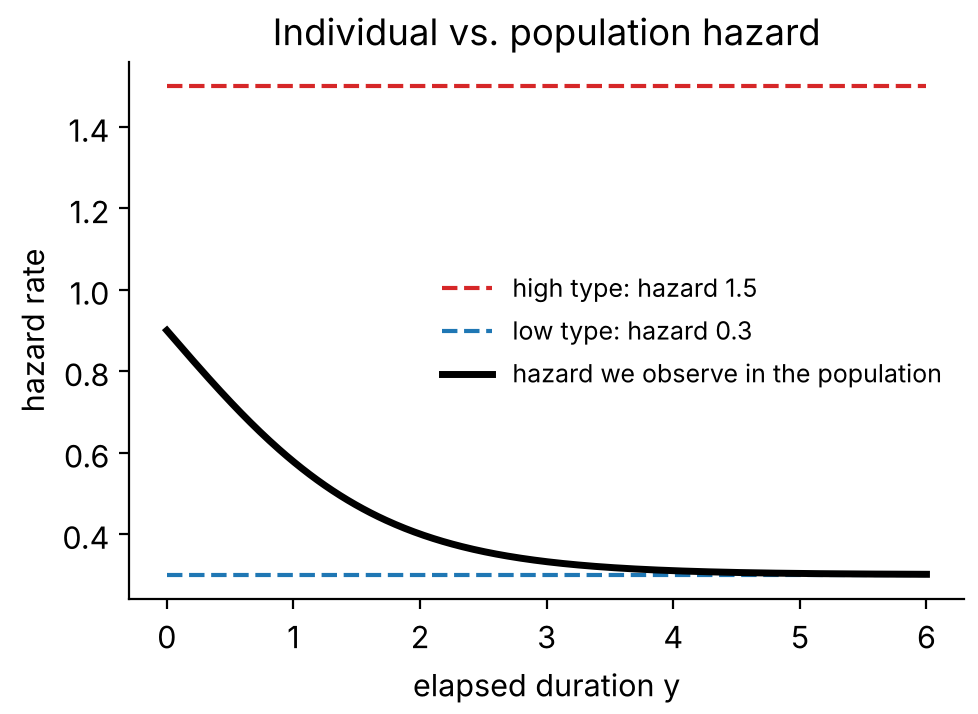
\includegraphics[width=\linewidth]{fig1a_population_hazard.png}

      {\scriptsize Two types, constant hazards. Nobody's hazard falls; the observed one does.}
    \end{column}
  \end{columns}
\end{frame}

% ---------------------------------------------------------------------
\begin{frame}{The Laplace transform: isolating the type distribution}
  \[ \Lap(a):=\E\big[e^{-aV}\big], \qquad \bar S(y)=\Lap\big(\Lambda(y)\big). \]
  \begin{itemize}
    \item $\Lap$ depends only on $G$; $\Lambda$ only on duration dependence.
    \item Survival = (heterogeneity) applied to (duration dependence).
  \end{itemize}
  \textbf{Properties}
  \begin{align*}
    -\frac{\Lap'(a)}{\Lap(a)} &= \E[V\mid\text{survived to }a] && \why{differentiate under $\E$} \\
    \frac{d^2}{da^2}\log\Lap(a) &= \var(V\mid\text{survived to }a) && \why{quotient rule} \\
    \Longrightarrow\ \frac{d}{dy}\E[V\mid Y>y] &= -\lambda(y)\var(V\mid Y>y)\ \le 0 && \why{chain rule}
  \end{align*}
  \begin{itemize}
    \item \textbf{Uniqueness:} $\Lap$ determines $G$.
    \item \textbf{Analyticity:} $\Lap$ on any small interval $\Rightarrow$ $\Lap$ everywhere.
    \item Strategy: learn the index, learn $\Lap$ on an interval $\Rightarrow$ $G$.
  \end{itemize}
\end{frame}

% ---------------------------------------------------------------------
\begin{frame}{Duration dependence or sorting? Not identified from one duration}
  \begin{columns}[T]
    \begin{column}{0.52\textwidth}
      \[ \bar\theta(y)=\underbrace{\lambda(y)}_{\text{duration dep.}}\cdot\underbrace{\E[V\mid Y>y]}_{\text{sorting}} \]
      \begin{itemize}
        \item Data: $\bar S(y)$ for all $y$.
        \item Unknowns: $\Lambda$ and $G$, with $\bar S(y)=\Lap_G(\Lambda(y))$.
        \item One data function, two unknown functions of the same $y$.
        \item Any $G$ fits: $\Lambda$ bends to absorb the rest.
      \end{itemize}
      \medskip
      \textbf{To separate them}, we need variation that moves one but not the other:
      \begin{itemize}
        \item groups at different stages of sorting, same $\lambda$;
        \item the same person observed twice;
        \item parametric restrictions on $\Lambda$ or $G$.
      \end{itemize}
    \end{column}
    \begin{column}{0.46\textwidth}
      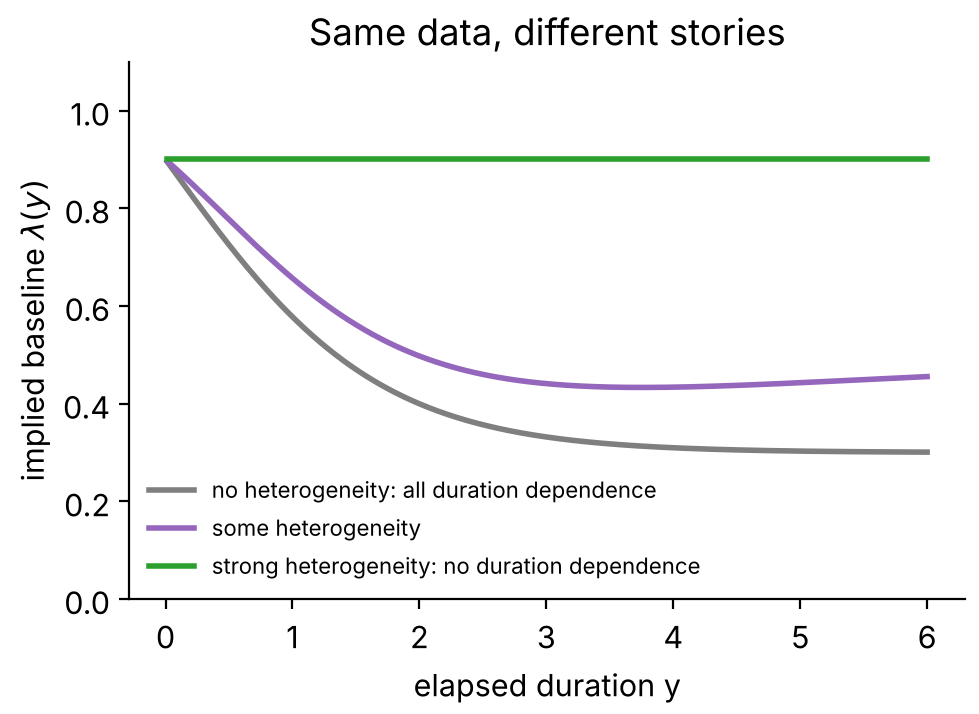
\includegraphics[width=\linewidth]{fig1b_same_data.png}

      {\scriptsize Same observed survival, three type distributions, three implied baselines.}
    \end{column}
  \end{columns}
\end{frame}

\end{document}
